\subsubsection{Geral}
Significa \textit{HyperText Markup Language} e define a \textbf{estrutura} e \textbf{significado} dos elementos de página web. Usando um prédio como comparação, o HTML seria as vigas, o cimento, os buracos para as janelas, os espaços para os encanamentos e fiação elétrica e etc.

HyperText se refere ao fato de muitas dessas páginas estarem ligadas umas as outras através de links, criando assim uma grande rede que compõe parte da World Wide Web.

Markup se refere ao fato de o texto HTML ser marcado por ``tags'' que definem os elementos usados na página. Vamos dar uma olhada em como isso é escrito na realidade:

\begin{figure}[h!]
    \centering
    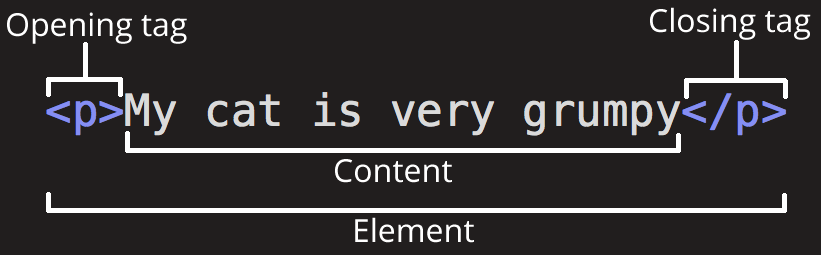
\includegraphics[scale=.4]{imgs/element-anatomy.png}
    \caption{Anatomia geral de um elemento HTML.}
    \label{fig:element-anatomy}
\end{figure}


\begin{itemize}
\item
  \textbf{tag de abertura:} é o nome do elemento envolvido por
  \texttt{\textless{}} à esquerda e por \texttt{\textgreater{}} à
  direita.
\item
  \textbf{tag de fechamento:} é o nome do elemento envolvido por
  \texttt{\textless{}/} à esquerda e por \texttt{\textgreater{}} à
  direita Note a presença da barra normal. Além disso, é válido
  mencionar que nem todos os elementos precisam de uma tag de
  fechamento. De maneira de geral quando ela não tem um conteúdo a tag
  de fechamento pode ser desconsiderada.
\item
  \textbf{conteúdo:} é o que vai entre as tags. Pode ser texto como na
  imagem ou até mesmo outros elementos como veremos mais pra frente.
\item
  \textbf{elemento =} tag de abertura \textbf{+} conteúdo \textbf{+} tag
  de fechamento (novamente, de maneira geral)
\end{itemize}

Para conhecer outros elementos, clique
\href{https://developer.mozilla.org/en-US/docs/Web/HTML/Element}{aqui}.


\subsubsection{Atributos}
Além disso, elementos HTML podem possuir atributos:

\begin{figure}[h!]
    \centering
    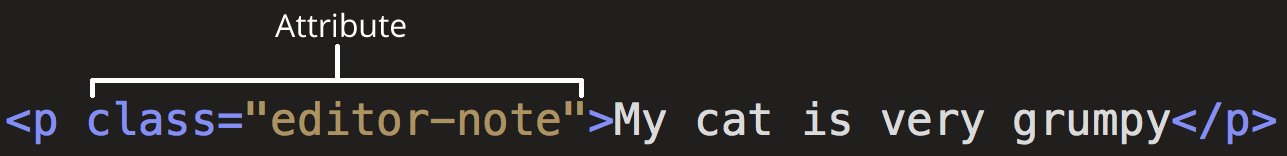
\includegraphics[scale=.3]{imgs/attrs.png}
    \caption{Anatomia geral de um elemento HTML.}
    \label{fig:attrs}
\end{figure}

Atributos são informações adicionais que passamos para os elementos.
Eles não aparecem no conteúdo. No caso da imagem, o atributo
\texttt{class} dá uma característica especial para esse elemento.
Veremos mais sobre \texttt{class} mais pra frente.


Vamos usar um editor de texto agora pra visualizar essas coisas. Crie
uma pasta chamada \texttt{matrix} no seu computador em um lugar que seja
conveniente pra você e abra essa pasta no seu editor. Para fazer isso,
geralmente é \emph{File} \textgreater{} \emph{Open Folder.}

Crie um arquivo \texttt{index.html} e abra-o no editor. Escreva o
seguinte:

\begin{figure}[h!]
    \centering
    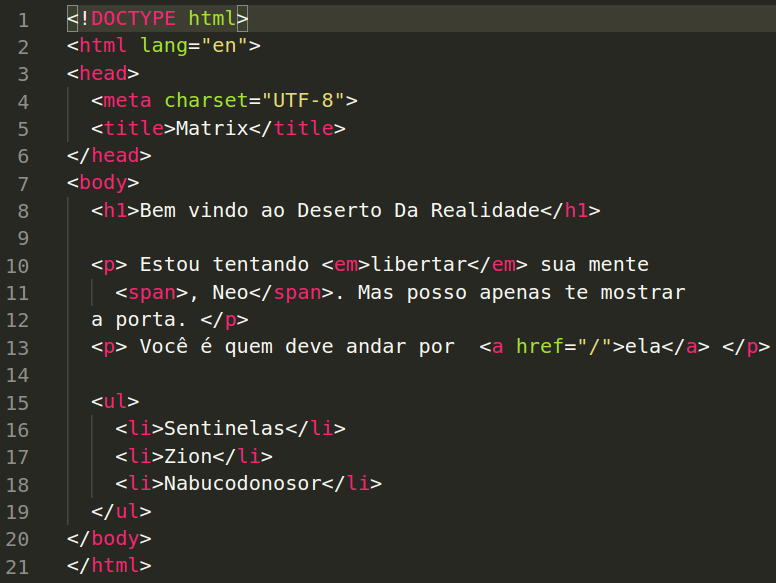
\includegraphics[scale=.4]{imgs/full-html-example.png}
    \caption{Exemplo de um código HTML completo.}
    \label{fig:full-html-example}
\end{figure}


No elemento \texttt{a} (link), \texttt{href} é outro tipo atributo que
indica ou ``vai'' para outra página ou recurso na internet.


\subsubsection{Visualização do HTML}
Podemos visualizar o resultado do que escrevemos de pelo menos duas
formas:

\begin{enumerate}
\item
  Abra o navegador de sua preferência (Chrome, Firefox, Edge) e arraste
  o arquivo \texttt{index.html} para o navegador. Se utilizarmos essa
  forma, temos que atualizar (\emph{a cada} alteração) a página do
  navegador para visualizarmos as alterações que fizermos no código.
\item
  Outra forma é utilizando uma extensão que existe para editores de
  texto. Essa extensão abre um servidor no nosso computador que escuta
  por alterações nos arquivos e atualiza a página automaticamente caso
  aconteçam.
\end{enumerate}

Para instalar o plugin no VSCode use o atalho \texttt{Ctrl+shift+x} (ou
clique no último ícone da barra lateral esquerda) para abrir a loja de
extensões e procure por Live Server e clique nela. Clique em ``Install''.
Você deve ver algo parecido com a Figura \ref{fig:live-server-ext}.

\begin{figure}[h!]
    \centering
    
\includegraphics[scale=.5]{imgs/live-server-extension.png}
    \caption{Foto da extensão.}
    \label{fig:live-server-ext}
\end{figure}

A loja de extensões no VS code é muito rica. Extensões servem para
ajudar o programador a programar seja corrigindo um trecho de código
automaticamente seja incorporando uma série de atalhos para geração
automática de código para algumas linguagens (para mais sugestões clique
nesse
\href{https://www.ubuntupit.com/best-visual-studio-code-extensions-for-programmers/}{link}).
Além dessas úteis, existem também algumas de zoerinha como a extensão
\href{https://marketplace.visualstudio.com/items?itemName=hoovercj.vscode-power-mode}{Power
Mode}.

\begin{figure}[h!]
    \centering
    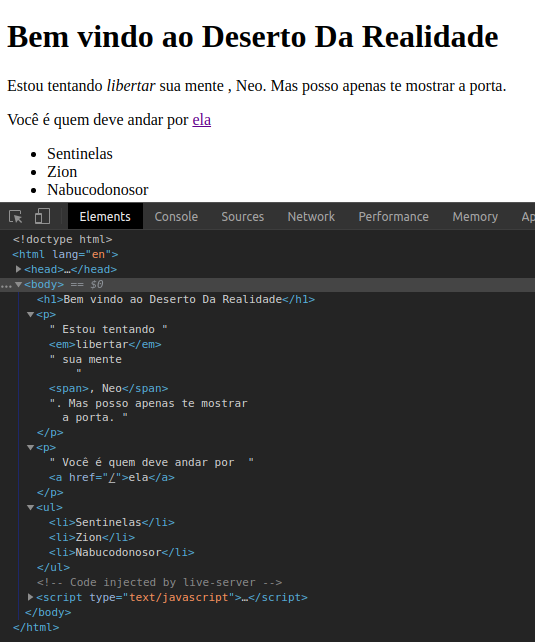
\includegraphics[scale=.5]{imgs/page-chr-dev-tools.png}
    \caption{HTML renderizado na página com o painel DevTools do Chrome aberto.}
    \label{fig:page-chr-dev-tools}
\end{figure}

No \textit{screenshot} da Figura \ref{fig:page-chr-dev-tools} podemos ver o resultado 
renderizado pelo navegador e logo embaixo a árvore de elementos que representa o que 
vemos na página. Essa árvore também é conhecida como árvore DOM (Document Object Model).
Veremos mais sobre ela mais pra frente.

Esse painel se chama Chrome DevTools. Para abri-lo basta apertar
\texttt{F12} ou clicar na página com o botão direito e ``Inspector''. Ou
ainda \texttt{Ctrl+c} pra abrir o inspecionador diretamente.

\newpage
\subsubsection{Anatomia do HTML}

Em programas C existe uma parte do código que sempre se repete, comumente conhecido como ``boilerplate'' em inglês. Em HTML isso também acontence. Vamos entender agora de maneira geral o que eles significam:

\begin{itemize}
\item
  \texttt{\textless{}!DOCTYPE\ html\textgreater{}}: indica que o tipo de
  documento (de fato não escrevemos até agora porque nosso projeto
  porque ele não tão necessário assim pra nós)
\item
  \texttt{\textless{}html\textgreater{}\textless{}/html\textgreater{}}:
  envolve todos os outros elementos
\item
  \texttt{\textless{}head\textgreater{}\textless{}/head\textgreater{}}:
  contém as informações necessárias para mostrar o conteúdo da página.
  Entretanto, o que está dentro de \texttt{head} não será visível.
\item
  \texttt{\textless{}meta\ charset="utf-8"\textgreater{}}: conjunto de
  caracteres gigante. É o que vai permitir a gente usar caracteres
  especiais e de outras línguas como a japonesa.
\item
  \texttt{\textless{}title\textgreater{}\textless{}/title\textgreater{}}:
  é o título da página na aba.
\item
  \texttt{\textless{}body\textgreater{}\textless{}/body\textgreater{}}:
  contém todo o conteúdo que pode ser visualizado pelo usuário final.
\end{itemize}

\textbf{Elementos inline} - não ocupam a linha toda. Exemplos:
\texttt{em}, \texttt{span}, \texttt{img}, \texttt{input},
\texttt{a}\ldots{} etc

\textbf{Nível block} - podem ser entendidos como um bloco que ocupa a
linha toda. Exemplos: \texttt{h1}, \texttt{h2}\ldots{} (e todos os
headings), \texttt{div}, \texttt{section}, \texttt{p}, \texttt{ul},
\texttt{li}\ldots{} etc.

Em termos práticos, podemos ver essa diferença na página do navegador na
qual está aberto o arquivo \texttt{index.html}. Elementos inline ocupam
a mesma linha que outros elementos no primeiro parágrafo, como
\texttt{em} e \texttt{span} e o \texttt{a} no segundo parágrafo. Os
elementos a nível de block naturalmente não ficam na mesma linha mesmo
que o conteúdo do elemento faça sobrar espaço na linha. Por exemplo, o
\texttt{h1} e os \texttt{p} ocupam a linha inteira e, por consequência,
não estão na mesma linha. Da mesma maneira, se houvesse uma segunda
lista \texttt{ul} ela estaria embaixo da primeira lista.

Mas só com o que vimos até agora, nossa página fica muito feia e sem
graça. Vamos deixá-la mais interessante.
